\documentclass[a4paper]{article}

\renewcommand{\contentsname}{Obsah} %rename ToC to Obsah
\renewcommand{\refname}{Literatura} %rename Bibliography to Literatura

%--------packages
\usepackage{graphicx} % images
\usepackage[hidelinks]{hyperref} %clickable links with no ugly box
\usepackage{amsmath} %complex notation
\usepackage{amsfonts}
\usepackage{mathtools}
\usepackage[affil-it]{authblk} %for affiliation in the title of the work
\usepackage[multiple]{footmisc} %to allow for multiple footnotes in the same place
\usepackage{caption}
\usepackage{subcaption} %for two images side to side

\usepackage[czech]{babel} %čeština

%
% \linespread{1.5}

\title{Barevné polarizační zobrazování pro bioaplikace}
\author{Prokop Beneš}
\affil{BBPROJ04 - Bakalářský projekt}
\author{Vedoucí práce: Ing. Lukáš Krauz, Ph.D.}
\affil{Katedra Radioelektroniky, \\Fakulta Elektrotechnická, \\České Vysoké Učení v Praze}
\date{\today}


\numberwithin{equation}{section}

\begin{document}
	\maketitle
	\newpage

	\tableofcontents
	\newpage

    \section{Úvod}
    Barevné polarizační zobrazování představuje inovativní přístup k analýze optických vlastností materiálů,
    který se stále více prosazuje v mnoha oborech, velké množství aplikací má takovéto měření v oborech technických, ale velké potenciální uplatnění má i v oborech biomedicínských.\cite{biomedical,spie} Využití polarizace světla umožňuje získávat informace o vlastnostech vzorků, které by jinak byly obvyklými metodami nepozorovatelné, a to například strukturální a povrchové vlastnosti. \cite{photonics}
    \par Tato práce si klade za cíl teoreticky zpracovat problematiku barevného polarizačního zobrazování zpohledu fyziky, popsat na jakém principu funguje obvyklé polarimetrické měření. Popsat jakým způsobem funguje barevný polarizační senzor IMX250MYR, který budeme používat na snímání polarizace. Ten je integrovaný v kameře BFS-U3-51S5PC-C. Popíšeme si jednoduchý způsob, kterým jsme schopni si snímek z naší kamery rozdělit do jednotlivých polarizovaných snímků. Nakonec si představíme na jaké různé využití se dá barevné polarizované zobrazování použít na konkrétních biomedicinských aplikacích.   \footnotemark[1]\footnotemark[2]\footnotemark[3]%\footnote{\url{https://www.flir.eu/globalassets/support/iis/knowledge-base/getting-started-with-bfs-polarized-cameras.pdf}} \footnote{\url{https://www.teledynevisionsolutions.com/learn/learning-center/machine-vision/imaging-reflective-surfaces-sonys-first-polarized-sensor/}} %\cite{flir,teledyne,senzor}
    \footnotetext[1]{\url{https://www.flir.eu/globalassets/support/iis/knowledge-base/getting-started-with-bfs-polarized-cameras.pdf}}
    \footnotetext[2]{\url{https://www.teledynevisionsolutions.com/learn/learning-center/machine-vision/imaging-reflective-surfaces-sonys-first-polarized-sensor/}}
    \footnotetext[3]{\url{https://www.sony-semicon.com/files/62/flyer_industry/IMX250_264_253MZR_MYR_Flyer_en.pdf}}
	\newpage
        
	\section{Polarizace}
    Elektromagnetické vlny mají velmi široký spektrální interval. My budeme uvažo-
    \\vat elektromagnetické vlnění pro nás viditelné. Tento interval elektromagnetického vlnění se nachází v intervalu přibližně 380 - 720nm. O elektromagnetickém vlnění v tomto intervalu budeme mluvit jako o světle. \cite{maly}
    \par Elektromagnetická postupná vlna je vlna příčná, což znamená, že elektrické a magnetické pole jsou kolmé na směr šíření. To znamená, že existuje dva nezávislé směry pro vektory těchto polí, mluvíme o dvou nezávislých My se zaměříme na popis elektrické složky vlny $\vec{E}$, protože vektor magnetické složky $\vec{B}$ je určena vztahem $\vec{B}= \frac{1}{v}\vec{s}\times\vec{E}$, kde $\vec{s}$ je vektor udávající směr šíření. Když zvolíme souřadný systém tak, že směr šíření je $\vec{s}=z$. Pak můžeme jako bázi příčné roviny, ve které se nachází $\vec{E}$, použít osy $x$ a $y$. Obecný vektor elektrického pole pak lze rozložit na složky směřující podél souřadných os.


    %dooznačit všechny proměnné!!!!!!!!!!!!!!!!!!!!!!!!!!!!!
    \begin{equation} \label{eq:1}
        \vec{E} = E_x\vec{x} + E_y\vec{y}
    \end{equation}
    Pokud budeme uvažovat harmonické postupné vlny, můžeme díky principu superpozice zvolit vlnu s různou amplitudou a s různým fázovým posunem:
    \begin{equation} \label{eq:2}
        \vec{E}(\vec{r},t) = E_{x0} e^{i(\omega t - kz + \varphi_1)} \vec{x} + 
                             E_{y0} e^{i(\omega t - kz + \varphi_2)} \vec{y}
    \end{equation}
    \par Fázový rozdíl těchto dvou složek můžeme vyjádřit jako 
    \begin{equation} \label{eq:3}
        \delta \varphi = (\omega t -kz + \varphi_1) - (\omega t -kz + \varphi_2) = \varphi_1 - \varphi_2
    \end{equation}
    ten nezávisí ani na čase ani na poloze v prostoru. Zvolíme si libovolné místo v prostoru jako $z = z_0$, můžeme sledovat časový průběh elektrického pole $\vec{E}(t) = \vec{E}(z_0,t)$
    \begin{equation} \label{eq:4}
        \vec{E}(t) = E_{x0} \vec{x} e^{i(\omega t + \varphi_1')} + E_{y0} \vec{y} e^{i(\omega t + \varphi_2')}
    \end{equation}
    kde $\varphi_i' = \varphi - kz_0$. Znovu tedy platí to samé pro rozdíl fází
    \begin{equation} \label{eq:5}
        \delta \varphi = \varphi_1 - \varphi_2 = \varphi_1' - \varphi_2' = (\varphi_1 - kz_0) - (\varphi_2 - kz_0)
    \end{equation}
    \par Z toho tedy vyplývá, že pro fázový rozdíl není důležité, ve kterém místě budeme průběh elektrického pole sledovat. Není třeba se zaobírat konrétními hodnotami fází, rozlišujeme pouze jejich rozdíl $\delta \varphi$.Reálná část rovnice (\ref{eq:4}) má tvar:
    \begin{equation} \label{eq:6}
        \vec{E}(t) = E_{x0}\vec{x}\cos(\omega t + \varphi_1) + E_{y0}\vec{y}\cos(\omega t + \varphi_2)
    \end{equation}
    je parametrickou rovnicí elipsy. Vektor elektrického pole $\vec{E}$ tedy v daném místě opisuje křivku, která má tvar elipsy. Tato elektromagnetická vlna je tedy elipticky polarizovaná. 
    \par Vlny tvaru (\ref{eq:4}), můžeme psát pomocí komplexního vektoru o dvou složkách $\hat{\vec{E}} \in \mathbb{C}^2$, 
    \begin{equation}
        \vec{E}(z,t) = \big(E_{x0} e^{i\varphi_1} \vec{x} + E_{y0} e^{i\varphi_2} \vec{y} \big)  e^{i(\omega t - kz)} = \hat{\vec{E}} e^{i(\omega t-kz)}
    \end{equation}
    \begin{equation}
        \hat{\vec{E}} = \begin{pmatrix} \hat{E}_1 \\ \hat{E}_2 \end{pmatrix} = \begin{pmatrix} E_{x0} \, e^{i \varphi_1} \\ E_{y0} \, e^{i \varphi_2} \end{pmatrix}	 \in \mathbb{C}^2
    \end{equation}
    \par Jeden pro nás velmi důležitý speciální případ je vlna, která je lineárně polarizovaná. Ta nastává, pokud vektor elektrické intenzity $\vec{E}$ kmitá jednom daném směru. 
    \par Tento případ nastává pro fázový posun $\delta \varphi \in \{0,\pi\}$, což pak můžeme zapsat jako
    \begin{equation} \label{eq:7}
        \vec{E} = E_0 \vec{n} e^{i(\omega t + \varphi]}
    \end{equation}
    neboli 
    \begin{equation} 
        \hat{\vec{E}} = E_0 \, \vec{n} \, e^{i\varphi} = E_0 \begin{pmatrix} \cos \theta \\ \sin \theta \end{pmatrix} e^{i\varphi}
    \end{equation}
    kde jednotkový vektor $\vec{n} = (n_x,n_y) = (\cos \theta, \sin \theta)$ znázorňuje směr kmitání elektrického pole $\vec{E}(t)$ v rovině $xy$ a úhel $\theta$ značí odklon tohoto vektoru od osy $x$. \cite{schmidt}
    \par Jedním z nejobvyklejších způsobů kde se v životě potkáme s polarizovaným světlem je bězná polarizace odrazem. Tento proces vychází ze Snellova zákona následujícím způsobem: 
    \begin{equation}
        n_1 \sin \theta_i = n_2 \sin \theta_t
    \end{equation}
    je Snellův zákon a $n_1$ a $n_2$ značí index lomu daného prostředí v kterém se světlo šíří.  $\theta_i$ je úhel dopadu, $\theta_t$ je úhel lomu. Úhlu pod kterým musí světlo dopadnout aby bylo lineárně polarizováno se říká úhel Brewsterův. 
    \begin{figure}[ht]
        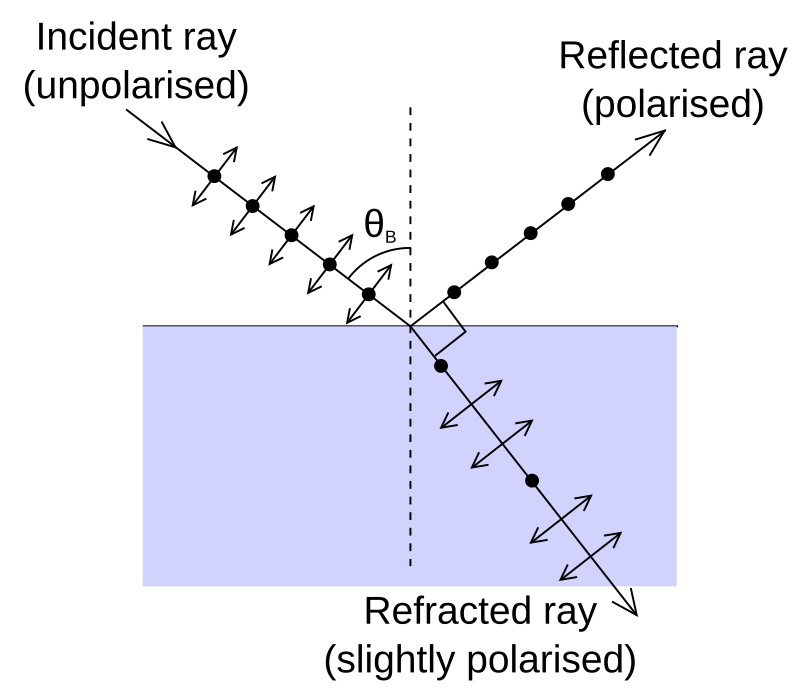
\includegraphics[width=7cm]{figures/Brewster.png}
        \centering
    \end{figure}
    \par Pro něj platí že $\theta_i + \theta_t = 90^{\circ}$, tedy, že úhel dopadajícího, tedy i odraženého světla musí svírat se světlem lomeným úhel devadesáti stupňů. Tedy $\theta_t = 90^{\circ} - \theta_i$ dosadíme do Snellova zákona. 
    \begin{equation}
        \!
        \begin{aligned}
            n_1 \sin \theta_i &= n_2 \sin (90^{\circ} - \theta_i) \\
            n_1 \sin \theta_i &= n_2 \cos \theta_i
        \end{aligned}
    \end{equation} 
    což nám po úpravě dá 
    \begin{equation}
        \frac{n_2}{n_1} = \frac{\sin \theta_i}{\cos \theta_i}
    \end{equation}
    neboli
    \begin{equation}
        \tan \theta_i = \frac{n_2}{n_1}
    \end{equation}
    Kde námi požadovaný Brewsterův úhel dostaneme jako
    \begin{equation}
        \theta_B = \arctan \frac{n_2}{n_1}
    \end{equation}
    Nepolarizované světlo dopadjící pod tímto úhlem se od rozhraní odráží pouze se složkou kolmou k rovině rozhraní. \cite{hecht} 
    \par Takto lineárně polarizované světlo pro nás bude v následujícím textu velmi důležité. Na princip lineárně polarizovaného světla totiž stojí princip naší barevné polarizované kamery BFS-U3-51S5PC-C
    \par Z polarizovaného světla jsme schopni, díky senzoru naší kamery, dostat zajímavé informace o předmětech, které budeme pozorovat. Na každý pixel superpixelu našeho senzoru dopadá světlo o dané intentitě $I_i$, kde nám $i$ značí orientaci polarizačního filtru před pixelem. Tedy $45^{\circ}, 0^{\circ},90^{\circ}, 135^{\circ}$. Tyto intenzity použijeme k zavedení Stokesova vektoru popisujícího polarizované světlo
    \begin{equation}
        S = \begin{bmatrix} S_0 \\ S_1 \\ S_2 \end{bmatrix} = \begin{bmatrix} I_0 + I_{90} \\ I_0 - I_{90} \\ I_{45} - I_{135} \end{bmatrix}
    \end{equation}
    \par Pomocí jednotlivých složek Stokesova vektoru si můžeme spočítat parametry snímku, které bychom jinak nezjistili. Jako první si určíme míru lineární polarizace, anglicky Degree of Linear Polarization (DoLP)
    \begin{equation}
        \text{DoLP} = \frac{\sqrt{S_1^2 + S_2^2}}{S_0}
    \end{equation}
    To nám říká, jaký podíl světla v daném pixelu je polarizovano.
    \par Další zajímavou informaci získatelnou ze složek Stokesova vektoru je úhel lineární polarizace, anglicky Angle of Linear Polarization (AoLP). Tento úhel nám říká jaký je průměrný úhel polarizace dopadajícího světla na daný pixel. \cite{teorie_aolp_dolp}
    \begin{equation}
        \text{AoLP} = \frac{1}{2}\arctan \left(\frac{S_2}{S_1}\right)
    \end{equation}

    \newpage
	\section{Aplikace Polarizace}
	Senzor kamery s kterou pracujeme má na svém senzoru mikrostrukturu, která se chová jako polarizátor přicházejícího světla, jelikož je jeho rozměr dostatečně malý na to, aby jím prošla jen určitá složka světla v daném úhlu podle úhlu samotného polarizátoru. Senzor samotný má každý pixel sestaven ze čtyř podpixelů kde každý z nich má přes sebe jiný úhel polarizátoru a to $90^{\circ}, 45^{\circ}, 135^{\circ}, 0^{\circ}$ podle směru hodinových ručiček začínaje vlevo v rohu.
    \begin{figure}[h]
        \includegraphics[width=8cm]{figures/senzor.jpg}
        \centering
    \end{figure}

    \subsection{Senzor Sony IMX250MYR}
    Kamera BFS-U3-51S5PC-C se senzorem Sony IMX250MYR, se kterou pracujeme, se již objevuje ve výzkumných publikacích využívajících polarizované snímání. Ať už z pohledu kalibrace samotného senzoru, nebo se také řeší demosaicing snímků získaných z tohoto senzoru, samozřejmě jsou publikovány i výzkumné články zkoumající chování polarizace za pomocí tohoto senzoru.\footnotemark[1]\cite{kalibrace,kalibrace2,aplikace} Z kamery lze dostat snímky díky poskytnutému softwaru. Zde si můžeme nastavit například white balance, expozici, kontrast nebo třeba gamma korekci. Získáme ze software kamery RAW fotku, kterou jsmě schopni zpracovat například v MATLABu s tím, že je potřeba foktu z RAW formátu upravit do formátu pro nás vhodného pro nějakopu další analýzu. Na to máme připravený krátký skript v MATLABu, nejprve je třeba si udělat demosaicing pomocí inbuilt matlab funkce "demosaic", která nám vrátí RGB snímek dekódovaný podle specifikovaného uspořádání Bayerovského filtru, který je v tomto případě RGGB.\footnotemark[2] Pokud chceme z kamery dostat celkový snímek je třeba tento demosaicovaný snímek po blocích zprůměrovat. Dále pokud budeme chtít snímky obsahující informace o polarizaci dané fotky tak je třeba si takovýto obrázek rozdělit na čtyři snímky s úhly polarizace podle toho z jaké části superpixelu si je vezmeme. Výsledkem tedy budou čtyři fotky, které obsahují pouze informace z těch daných úhlů samotných pixelů. Z těch jsme poté, pomocí například Stokesových parametrů, určit Degree of Linear Polarization (DoLP) a nebo Angle of Linear Polarization (AoLP). Tyto parametry nám mohou poskytnout důležité informace lidským okem  nepozorovatelné.\footnotemark[3]

    \footnotetext[1]{\url{https://www.mathworks.com/matlabcentral/fileexchange/131763-demosaicing-algorithm-for-sony-imx250myr}}
    \footnotetext[2]{\url{https://www.mathworks.com/help/images/ref/demosaic.html}}
    \footnotetext[3]{\url{https://www.sony-semicon.com/en/technology/industry/polarsens.html}}


    \subsection{Využití polarizace ve výzkumu}
    Specifických využití polarizačního zobrazování je veliké množství a proto si ukážeme jen některé obecné zajímavé aplikace, včetně možným aplikacím v oblasti biologie a biomedicíny. Možností použití polarizačního barevného senzoru, je díky jeho schopnosti snímat i polarizované barevmé snímky, velmi zajímavé. Pomocí polarizace jsem schopni ze snímků dostat informace, které by bylo za použití konvenčních metod snímání velmi náročné. To ať už kvůli odrazivosti materiálů materiálů které snímáme, nebo světelných podmínek za kterých snímáme. Takovou aplikací může být například výrobní linka léků. Normální snímání samotných balení s léky může být náročné, když se jedná o prášky bílé na hliníkové fólii. Pak nám na rozpoznávání naplňěnosti balení, které chceme snímat kamerou, usnadní polarizační senzor. Díky rozdílu DoLP výrazně jednodušeji rozpoznáme zda v daném místě balení léků jeden chybí nebo ne.\footnotemark[1]

    \begin{figure}[h]
        \centering
        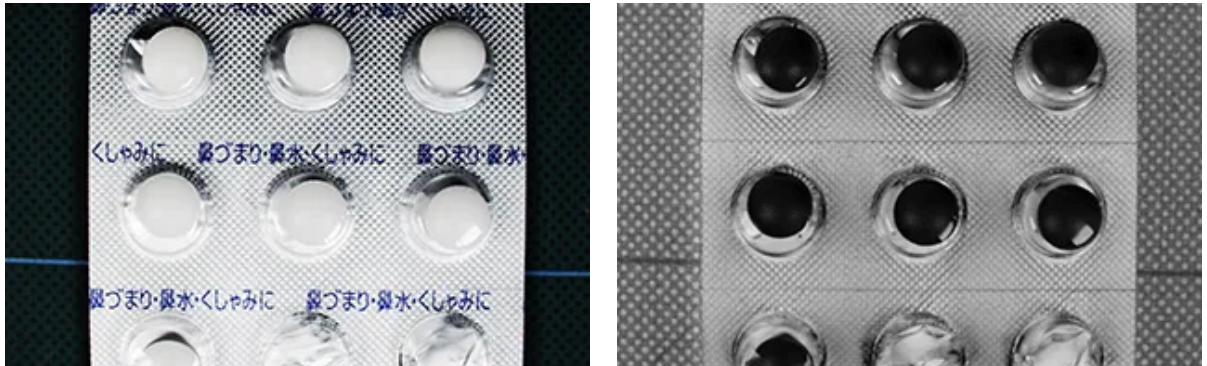
\includegraphics[width=8cm]{figures/pills.png}
        \caption*{Nepolarizované a polarizované balení léků}
    \end{figure}

    \par Dalším možným využitím polarizačního zobrazování je při zkoumání průhle-
    \\dných materiálů. Při zkoumání průhledných materiálů a objektů nám toho opět standardní senzory hodně neřeknou. Zato polarizační zobrazování nám poskytne díky AoLP nebo DoLP spoustu informací okem také nepozorovatelných. Například vnitřní napětí takovýchto objektů je bez polarizace nepozorovatelné, ale díky AoLP jsme jej schopni pozorovat i měřit.\footnotemark[2]
    \par Další zajímavé využití polarizačního snímání bude měření koncentrací různ-\\ých roztoků, například vodných roztoků cukrů. Jelikož je cukr chirální, tedy prostorově asymetrický, mění tedy optické vlastnosti roztoku a tedy i světla jím procházejícím. \cite{chiralita} Tyto změny jsme díky změně v polarizaci schopni pozorovat polarizační kamerou. K takovému měření budeme potřebovat Stokesovy parametry ze kterých si jsme schopni vypočítat AoLP. Úhel lineární polarizace nám právě o koncentraci roztoku poví co nás zajímá. Zobrazení tohoto úhlu polarizace je důležité, protože jsme díky němu schopni porovnat proti sobě různé koncentrace cukernatých roztoků, které bychom bez polarizační kamery nezjistili.\footnotemark[3]
    \begin{figure}[htbp]
        \centering
        \begin{subfigure}[h]{0.35\textwidth}
            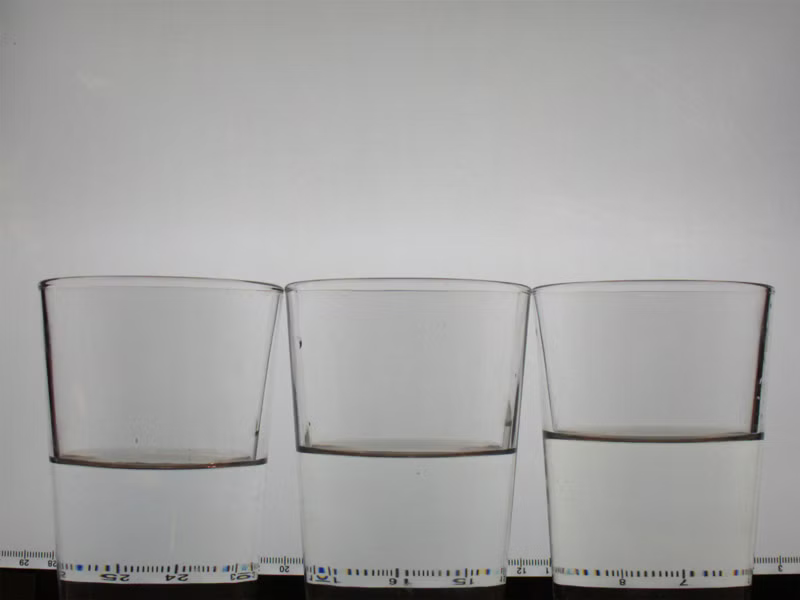
\includegraphics[width=\textwidth]{figures/Sugar-Water-Non-Polarized-Image.png}
            \caption{Nepolarizovaný roztok vody s cukrem}
        \end{subfigure}
        \hfill
        \begin{subfigure}[h]{0.35\textwidth}
            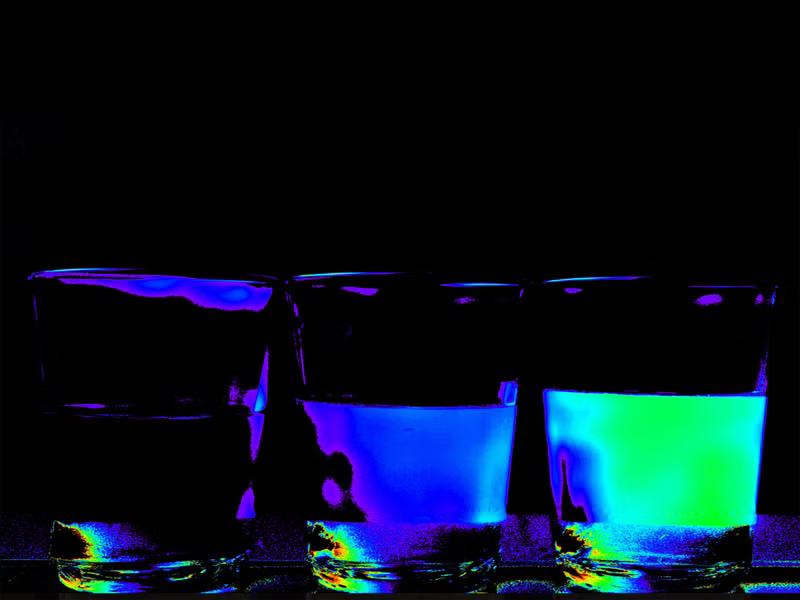
\includegraphics[width=\textwidth]{figures/Sugar-Water-Polarized-Image.png}
            \caption{AoLP roztoku vody s cukrem}
        \end{subfigure}
    \end{figure}

    \footnotetext[1]{\url{https://www.sony-semicon.com/en/technology/industry/polarsens.html}}
    \footnotetext[2]{\url{https://thinklucid.com/tech-briefs/polarization-explained-sony-polarized-sensor/}}
    \footnotetext[3]{\url{https://thinklucid.com/polarized-camera-resource-center/evaluating-sugar-concentration-in-water/}}

    \newpage
    \subsection{Závěr}
    V této práci jsme si představili současné a nadcházející možnosti využití polarizace v technických a biomedicinských aplikacích. Vytvořili jsme si teoretický základ, na kterém polarizace světla funguje a na jakém principu se dá polarizované světlo snímat. Pro analýzu polarizačních snímků jsme si popsali krátký skript v MATLABu pomocí kterého jsme schopni si ukázat různé úhly polarizace snímané naším senzorem. Dále jsme se věnovali detailnějšímu popisu jednotlivých aplikací polarimetrických měření.
    \par Na takto představený teoretický a aplikační základ můžeme navázat mnoha způsoby. Teoreická stránka této problematiky může být rozvinuta do většího detailu například po fyzikální stránce, nebo po stránce polarimetrické, která je více aplikovatelná. Mezi potenciální aplikace bychom mohli zkoumat polarimetrické měření koncentrací cukernatých roztoků, tedy s jakými vlastnostmi se mění optické vlastnosti roztoku se změnou koncentrace cukru ve vodě. 

    \newpage
    \addcontentsline{toc}{section}{Literatura}
    \begin{thebibliography}{99}
        \bibitem{biomedical} \textit{Optical Polarization in Biomedical Applications} \url{https://link.springer.com/book/10.1007/978-3-540-45321-5}
        \bibitem{spie} \textit{Polarized light imaging in biomedicine: emerging Mueller matrix methodologies for bulk tissue assessment} \url{https://www.spiedigitallibrary.org/journals/journal-of-biomedical-optics/volume-20/issue-6/061104/Polarized-light-imaging-in-biomedicine--emerging-Mueller-matrix-methodologies/10.1117/1.JBO.20.6.061104.full}
        \bibitem{photonics} \textit{Polarization-Based Imaging: Basics and Benefits} \url{https://www.photonics.com/Articles/Polarization-Based_Imaging_Basics_and_Benefits/a60734}
        %\bibitem{flir} \url{https://www.flir.eu/globalassets/support/iis/knowledge-base/getting-started-with-bfs-polarized-cameras.pdf}
        %\bibitem{teledyne} \url{https://www.teledynevisionsolutions.com/learn/learning-center/machine-vision/imaging-reflective-surfaces-sonys-first-polarized-sensor/}
        %\bibitem{senzor} \url{https://www.sony-semicon.com/files/62/flyer_industry/IMX250_264_253MZR_MYR_Flyer_en.pdf}
        \bibitem{maly} Malý P., \textit{Optika}, Nakladatelství Karolinum, 2008
        \bibitem{schmidt} Schmidt J., \textit{Vlnění, optika a atomová fyzika}, \url{https://physics.fjfi.cvut.cz/~schmijos/voaf/skriptaVOAF.pdf}
        \bibitem{hecht} Hecht E., \textit{Optics}, 4th Ed, Pearson, 2002
        \bibitem{teorie_aolp_dolp} Detection Limits for Chiral Amino Acids Using a Polarization Camera
        Claire Cook, Shane Byrne, Christian Drouet d'Aubigny, Donna Viola, Jill Mikucki and Walther Ellis, 2020, The Planetary Science Journal, Volume 1, Number 2 DOI: 10.3847/PSJ/abae57
        \url{https://iopscience.iop.org/article/10.3847/PSJ/abae57}
        \bibitem{kalibrace} C. Lane, D. Rode, and T. Rösgen, "Calibration of a polarization image sensor and investigation of influencing factors," Appl. Opt.  61, C37-C45 (2022). \url{https://opg.optica.org/ao/fulltext.cfm?uri=ao-61-6-C37&id=462441}
        \bibitem{kalibrace2} J. Rodriguez, L. Lew-Yan-Voon, R. Martins and O. Morel, "A Practical Calibration Method for RGB Micro-Grid Polarimetric Cameras," in IEEE Robotics and Automation Letters, vol. 7, no. 4, pp. 9921-9928, Oct. 2022, doi: 10.1109/LRA.2022.3192655. \url{https://ieeexplore.ieee.org/document/9834097}
        %\bibitem{demosaicing} \url{https://www.mathworks.com/matlabcentral/fileexchange/131763-demosaicing-algorithm-for-sony-imx250myr}
        \bibitem{aplikace} J. Marco-Rider, L. Tingelstad and O. Egeland, "Polarization image sensor-based laser scanner for reflective metals: architecture and implementation," 2021 IEEE Sensors, Sydney, Australia, 2021, pp. 1-4, doi: 10.1109/SENSORS47087.2021.9639607. \url{https://ieeexplore.ieee.org/stamp/stamp.jsp?tp=&arnumber=9639607}
        %\bibitem{matlab} \url{https://www.mathworks.com/help/images/ref/demosaic.html}
        %\bibitem{aolp} \url{https://www.sony-semicon.com/en/technology/industry/polarsens.html}
        %\bibitem{stresy} \url{https://thinklucid.com/tech-briefs/polarization-explained-sony-polarized-sensor/}
        \bibitem{chiralita}  Sweet chirality: the taste of l- and d-glucose stereoisomers
        Nitzan Dubovski, Yaron Ben Shoshan-Galeczki, Einav Malach, Masha Y Niv
        bioRxiv 2020.08.16.252718; doi: https://doi.org/10.1101/2020.08.16.252718 \url{https://www.biorxiv.org/content/10.1101/2020.08.16.252718v1.full.pdf}
        %\bibitem{sugar} \url{https://thinklucid.com/polarized-camera-resource-center/evaluating-sugar-concentration-in-water/}
    \end{thebibliography}
\end{document}